% \documentclass[fleqn]{article}
%\documentclass[twocolumn,10pt]{article}
\documentclass[nocopyrightspace,10pt]{sigplanconf}

\usepackage{xspace,amsmath,math-cmds,
            math-envs,inference-rules,times,
            verbatim,alltt,multicol,proof,url}
\usepackage{epsfig}
\usepackage{code} 
%\setlength{\oddsidemargin}{0in}
%\setlength{\evensidemargin}{0in}
%\setlength{\textwidth}{6.5in}
%\setlength{\textheight}{8.5in}

\setlength{\hoffset}{-1in}
\setlength{\voffset}{-1in}

\setlength{\topmargin}{.5in}
\setlength{\headheight}{0pt}
\setlength{\headsep}{0pt}

\setlength{\evensidemargin}{.75in}
\setlength{\oddsidemargin}{.75in}

% Text area:

\newdimen{\standardtextwidth}
\setlength{\standardtextwidth}{42pc}

\setlength{\textwidth}{\standardtextwidth}

\setlength{\topskip}{0pt}
\setlength{\columnsep}{1.5pc}
\setlength{\textheight}{59pc}
\newcommand{\cut}[1]{}
\newcommand{\reminder}[1]{{\it #1 }}
\newcommand{\edcom}[1]{\textbf{{#1}}}
\newcommand{\poplversion}[1]{#1}
\newcommand{\trversion}[1]{}

\newcommand{\appref}[1]{Appendix~\ref{#1}}
\newcommand{\secref}[1]{Section~\ref{#1}}
\newcommand{\tblref}[1]{Table~\ref{#1}}
\newcommand{\figref}[1]{Figure~\ref{#1}}
\newcommand{\listingref}[1]{Listing~\ref{#1}}
%\newcommand{\pref}[1]{{page~\pageref{#1}}}

\newcommand{\eg}{{\em e.g.}}
\newcommand{\cf}{{\em cf.}}
\newcommand{\ie}{{\em i.e.}}
\newcommand{\etal}{{\em et al}}
\newcommand{\etc}{{\em etc.\/}}
\newcommand{\naive}{na\"{\i}ve}
\newcommand{\role}{r\^{o}le}
\newcommand{\forte}{{fort\'{e}\/}}
\newcommand{\appr}{\~{}}

\newcommand{\bftt}[1]{{\ttfamily\bfseries{}#1}}
\newcommand{\kw}[1]{\bftt{#1}}
\newcommand{\pads}{\textsc{pads}}
\newcommand{\padsc}{\textsc{pads/c}}
\newcommand{\padx}{\textsc{padx}}
\newcommand{\ipads}{\textsc{ipads}}
\newcommand{\ir}{\textsc{IR}}
\newcommand{\padsl}{\textsc{padsl}}
\newcommand{\padsml}{\textsc{pads/ml}}
%\newcommand{\padsd}{\textsc{pads/d}}
\newcommand{\learnpads}{{\textsc{learnpads}}}
\newcommand{\padsd}{\textsc{Gloves}}
\newcommand{\blt}{\textsc{blt}}
\newcommand{\ddc}{\textsc{ddc}}
\newcommand{\ddl}{\textsc{ddl}}
\newcommand{\C}{\textsc{C}}
\newcommand{\perl}{\textsc{Perl}}
\newcommand{\ml}{\textsc{ml}}
\newcommand{\smlnj}{\textsc{sml/nj}}
\newcommand{\ocaml}{\textsc{OCaml}\xspace}
\newcommand{\haskell}{\textsc{haskell}\xspace}
\newcommand{\ocamlbig}{\textsc{OCAML}\xspace}
\newcommand{\java}{\textsc{java}}
\newcommand{\xml}{\textsc{xml}}
\newcommand{\html}{\textsc{html}}
\newcommand{\xpath}{\textsc{xpath}}
\newcommand{\xquery}{\textsc{xquery}}
\newcommand{\datascript}{\textsc{datascript}}
\newcommand{\packettypes}{\textsc{packettypes}}
\newcommand{\erlang}{\textsc{Erlang}}
\newcommand{\camlp}{\cd{Camlp4}}
\newcommand{\ocamlnet}{\cd{Ocamlnet} \cd{2}}

\newcommand{\totalcost}[2]{\textsc{Cost}(#1,#2)}
\newcommand{\costdescription}[1]{\textsc{CT}(#1)}
\newcommand{\normcostdescription}{\textsc{NCT}}
\newcommand{\costdata}[2]{\textsc{CD}(#2 \; | \; #1)}
\newcommand{\acostdata}[2]{\textsc{ACD}(#2 \; | \; #1)}
\newcommand{\adc}[2]{\textsc{CD'}(#2 \; | \; #1)}
\newcommand{\cardt}{\textsc{Card}}
\newcommand{\costvar}[1]{\textsc{CV}(#1)}
\newcommand{\costchar}[1]{\textsc{CA}(#1)}
\newcommand{\coststring}[1]{\textsc{CS}(#1)}
\newcommand{\costint}[1]{\textsc{CI}(#1)}
\newcommand{\costparam}[1]{\textsc{CP}(#1)}
\newcommand{\costconst}[1]{\textsc{CC}(#1)}

\newcommand{\dibbler}{Sirius}
\newcommand{\ningaui}{Altair}
\newcommand{\darkstar}{Regulus}

\newcommand{\vizGems}{Arrakis}

\newcommand{\comon}{CoMon\xspace}
\newcommand{\planetlab}{PlanetLab\xspace}
\newcommand{\monall}{Monall\xspace}
%% \newcommand{}{}


%% \newcommand{\IParray}[4]{{\tt Parray} \; #1 \; \[#2, #3, #4\]}

\newcommand{\figHeight}[4]{\begin{figure}[tb]
	\centerline{
	            \epsfig{file=#1,height=#4}}
	\caption{#2}
	\label{#3}
	\end{figure}}

\newcommand{\myalt}{\ensuremath{\; | \;}}
\newcommand{\normal}[1]{\ensuremath{\bar{#1}}}
\newcommand{\relativee}[2]{\ensuremath{{\cal R}(#1 \; || \; #2)}}
\newcommand{\srelativee}[2]{\ensuremath{{\cal S}(#1 \; || \; #2)}}
\newcommand{\addh}[2]{\ensuremath{#1 \oplus #2}}

\newcommand{\irstruct}[1]{{\tt struct}\{#1\}}
\newcommand{\irunion}[1]{{\tt union}\{#1\}}
\newcommand{\irenum}[1]{{\tt enum}\{#1\}}
\newcommand{\irarray}[1]{{\tt array}\{#1\}}
\newcommand{\irarrayFW}[2]{{\tt arrayFW}\{#1\}[#2]}
\newcommand{\irswitch}[2]{{\tt switch}(#1)\{#2\}}
\newcommand{\iroption}[1]{{\tt option}\{#1\}}
\newcommand{\setof}[1]{\lsem #1 \rsem}
\newcommand{\goto}{\Rightarrow}
\newcommand{\Pvoid}{{\tt Pvoid}}
\newcommand{\Pempty}{{\tt Pempty}}
\newcommand{\sskip}{\hspace*{5mm}}
\newcommand{\shrink}{\vspace*{-4mm}}

% Semantics
\newcommand{\setalt}{{\; | \;}}
\newcommand{\denote}[1]{\lsem #1 \rsem}
\newcommand{\lsem}{{[\![}}
\newcommand{\rsem}{{]\!]}}
\newcommand{\turn}{\vdash}
\newcommand{\meta}{m}
\newcommand{\nested}{n}
\newcommand{\mytime}[1]{#1.t}
\newcommand{\myds}[1]{#1.ds}
\newcommand{\myval}[1]{#1.nest}
\newcommand{\generatedloc}{\ensuremath{\mathtt{nowhere}}}
\newcommand{\environment}{E}
\newcommand{\universe}{U}
\newcommand{\selectOne}{\ensuremath{\mathsf{earliest}}}
% core feed semantics
\newcommand{\csemantics}[3]{{\cal C}\lsem #1 \rsem_{{#2} \, {#3}}}
% feed semantics
\newcommand{\semantics}[3]{{\cal F}\lsem #1 \rsem_{{#2} \, {#3}}}
% expression semantics
\newcommand{\esemantics}[2]{{\cal E}\lsem #1 \rsem_{{#2}}}
%\newcommand{\esemantics}[2]{#2(#1)}

% Host language types
\newcommand{\ty}{\ensuremath{\tau}}
\newcommand{\basety}{\ensuremath{b}}
\newcommand{\arrow}{\rightarrow}
\newcommand{\optionty}[1]{\ensuremath{#1 \; \mathsf{option}}}
\newcommand{\listty}[1]{\ensuremath{#1 \; \mathsf{list}}}
\newcommand{\setty}[1]{\ensuremath{#1 \; \mathsf{set}}}
\newcommand{\feedty}[1]{\ensuremath{#1 \; \mathsf{feed}}}
\newcommand{\corety}[1]{\ensuremath{#1 \; \mathsf{core}}}
\newcommand{\schedulety}{\ensuremath{\mathsf{sched}}}
\newcommand{\timety}{\ensuremath{\mathsf{time}}}
\newcommand{\locty}{\ensuremath{\mathsf{loc}}}
\newcommand{\boolty}{\ensuremath{\mathsf{bool}}}
\newcommand{\unitty}{\ensuremath{\mathsf{unit}}}
\newcommand{\stringty}{\ensuremath{\mathsf{string}}}
\newcommand{\metatype}[1]{\ensuremath{\mathsf{meta}(#1)}}
\newcommand{\nestedtype}[1]{\ensuremath{\mathsf{nest}(#1)}}
\newcommand{\dsty}{\ensuremath{\mathsf{ds}}}

\newcommand{\dom}{\ensuremath{\mathsf{dom}}}
\newcommand{\ueq}[3]{\ensuremath{#1 =_{#2} #3}}
\newcommand{\fsubset}[3]{\ensuremath{#1 \subseteq_{#2} #3}}
\newcommand{\feq}[3]{\ensuremath{#1 =_{#2} #3}}

% Expressions
\newcommand{\expression}{e}
\newcommand{\constant}{c}
\newcommand{\ds}{\ensuremath{ds}}
\newcommand{\boolf}{\ensuremath{\mathtt{false}}}
\newcommand{\boolt}{\ensuremath{\mathtt{true}}}
\newcommand{\loc}{\ensuremath{\ell}}
\newcommand{\feed}{\ensuremath{F}}
\newcommand{\corefeed}{\ensuremath{C}}
\newcommand{\generalvar}{\ensuremath{x}}
\newcommand{\feedvar}{\ensuremath{x}}
\newcommand{\itemvar}{\ensuremath{x}}
\newcommand{\data}{\ensuremath{v}}
\newcommand{\atime}{\ensuremath{t}}
\newcommand{\astring}{\ensuremath{w}}
\newcommand{\unit}{\ensuremath{()}}
\newcommand{\schedule}{\ensuremath{s}}
\newcommand{\parser}{\ensuremath{p}}
\newcommand{\none}{\ensuremath{\mathtt{None}}}
\newcommand{\some}[1]{\ensuremath{\mathtt{Some}\; #1}}
\newcommand{\inl}[1]{\ensuremath{\mathtt{inl}\; #1}}
\newcommand{\inr}[1]{\ensuremath{\mathtt{inr}\; #1}}
\newcommand{\casedata}[2]{{\tt switch}(#1)\{#2\}}
%\newcommand{\nillist}{\ensuremath{\mathtt{nil}}}
\newcommand{\nillist}{\ensuremath{[\,]}}
%\newcommand{\conslist}[2]{\ensuremath{\mathtt{cons} (#1,#2)}}
\newcommand{\conslist}[2]{\ensuremath{[#1,\ldots,#2]}}
\newcommand{\nilstream}{\ensuremath{\mathtt{done}}}
\newcommand{\consstream}[2]{\ensuremath{\mathtt{next} (#1,#2)}}


% Feeds
\newcommand{\comprehensionfeed}[3]{\ensuremath{\mathtt{\{|} #1 \; \mathtt{|}\; #2 \leftarrow #3 \mathtt{|\}}}}
\newcommand{\computed}[3]{\ensuremath{\mathtt{[} #1 \; \mathtt{|}\; #2 \in #3 \mathtt{]}}}
\newcommand{\letfeed}[3]{\ensuremath{\mathtt{let}\; #1 \; \mathtt{=}\; #2 \; \mathtt{in} \; #3}}
\newcommand{\allfeed}[5]{
  \ensuremath{
    \mathtt{all \{ format=} #1; 
    \mathtt{src=} #2;
    \mathtt{sched=} #3;
    \mathtt{pp=} #4;
    \mathtt{win=} #5;
  \mathtt{\}}}}
\newcommand{\existsfeed}[5]{
  \ensuremath{
    \mathtt{any \{ format=} #1; 
    \mathtt{src=} #2;
    \mathtt{sched=} #3;
    \mathtt{pp=} #4;
    \mathtt{win=} #5;
  \mathtt{\}}}}
\newcommand{\filterfeed}[2]{
  \ensuremath{
    \mathtt{filter} \; #1 \; \mathtt{with}\; #2}}
\newcommand{\remapfeed}[2]{
  \ensuremath{
    \mathtt{redirect} \; #1 \; \mathtt{with}\; #2}}
\newcommand{\ppfeed}[2]{
  \ensuremath{
    \mathtt{pp} \; #1 \; \mathtt{with}\; #2}}
\newcommand{\foreachupdate}[3]{
  \ensuremath{
    \mathtt{foreach{*}{*}}\; #1 \;
    \mathtt{in}\; #2 \;
    \mathtt{update}\; #3}}
\newcommand{\foreachcreate}[3]{
  \ensuremath{
    \mathtt{foreach*}\; #1 \;
    \mathtt{in}\; #2 \;
    \mathtt{create}\; #3}}
\newcommand{\remap}[2]{\ensuremath{\mathtt{redirect}\; #1 \; \mathtt{with} \; #2}}
\newcommand{\stutterfeed}[2]{\ensuremath{\mathtt{stutter}\; #1 \; \mathtt{on} \; #2}}
\newcommand{\refeed}[2]{\ensuremath{\mathtt{reschedule}\; #1 \; \mathtt{to} \; #2}}
\newcommand{\emptyfeed}{\ensuremath{\emptyset}}
\newcommand{\onefeed}[2]{\ensuremath{\mathtt{One}}(#1,#2)}
\newcommand{\sfeed}[1]{\ensuremath{\mathtt{SchedF}}(#1)}
\newcommand{\lfeed}[1]{\ensuremath{\mathtt{ListF}}(#1)}
\newcommand{\unionfeed}{\ensuremath{\cup}}
\newcommand{\sumfeed}{\ensuremath{+}}
\newcommand{\spairfeed}{\; \ensuremath{\mathtt{\&} \; }}
\newcommand{\allpairfeed}{\; \ensuremath{{*}{*}} \; }

\newcommand{\Time}{\ensuremath{\mathtt{Time}}}
\newcommand{\Set}{\ensuremath{\mathtt{Set}}}

% this is used for the translations equal
\newcommand{\transeq}{\stackrel{def}{=} }
\newcommand{\ai}{{\tt wl}}



% BNF
%\newcommand{\bnfalt}{\ |\ }


\begin{document}

\title{Typing Directory Structures\thanks{There are no student authors.  If
    accepted, Kathleen will make the presentation.}}

\authorinfo{Kathleen Fisher}
	   {AT\&T Labs Research}
           {\small \tt kfisher@research.att.com}
\authorinfo{David Walker}
	   {Princeton University}
           {\small \tt dpw@cs.princeton.edu}
\authorinfo{Kenny Q. Zhu}
	   {Princeton University}
           {\small \tt kzhu@cs.princeton.edu}

\maketitle{}


Many applications, be they single programs or collections of programs,
rely on a set of files, directories, and symbolic links to
store and organize information.  Examples include monitoring
systems, such as those developed for PlanetLab or internally at AT\&T;
version control systems such as CVS or SVN; repositories of scientific
data; test regression systems; mail and web page caches; software
package management systems; source code management systems, \etc{}

These applications assume that the constituent files, directories, and
symbolic links satisfy various properties, \eg{}, files and
directories must exist with appropriate owners, groups, and
permissions; symbolic links must have the correct targets; create
and/or modify times must be consistent, \etc{}  Privacy or hygiene
considerations might require that only a specified set of files exist.
Finally, index or configuration files may specify the directory and
file structure required by the application.  For example, CVS uses 
\cd{Entries} files to list the files and directories under source code
control:  

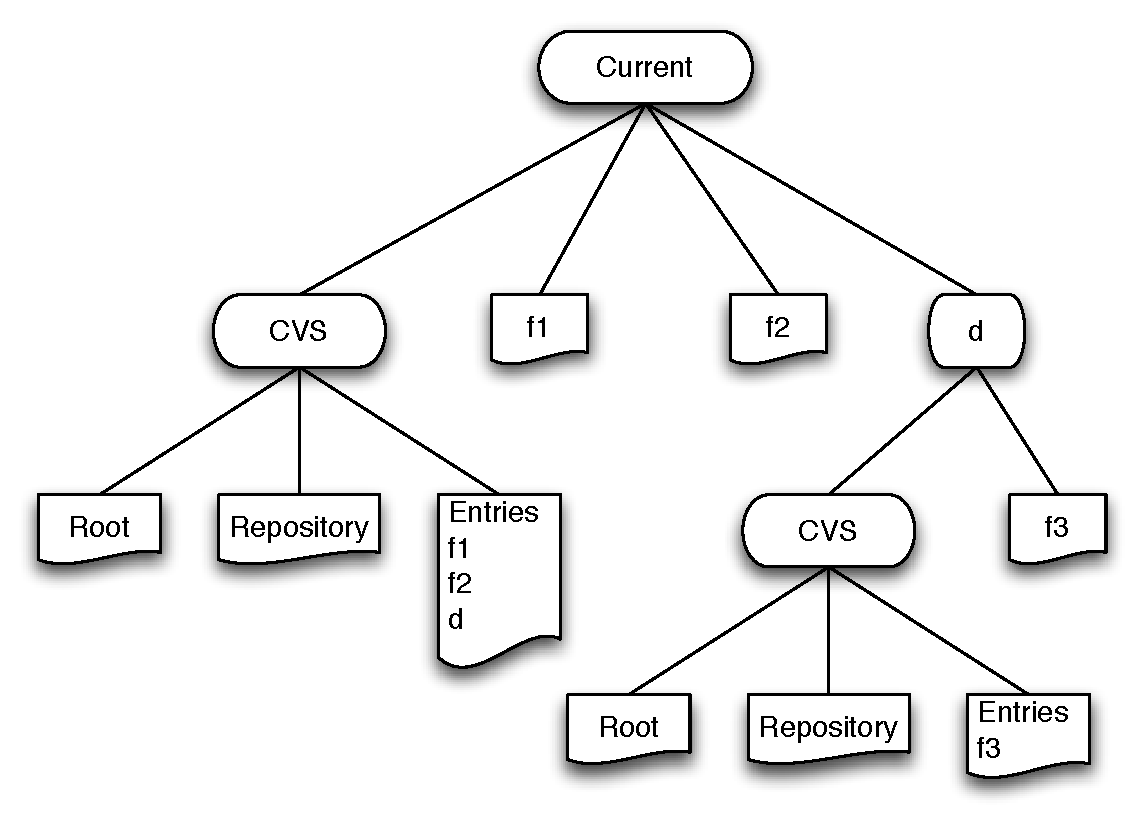
\includegraphics[scale=.4]{CVSStructure.pdf}
%width=\columnwidth]

If these properties fail to hold, applications can fail in
unpredictable ways with poor error messages.  Yet, general-purpose
tools to determine whether the portions of a file system specific to a
particular application are in a good state do not exist.  Instead, each
application writer must craft one-off tools or simply hope that errors
do not arise. 

To address this deficiency, we are designing \dirpads{}, a type-based
language 
for specifying the files, directories, and symbolic links that
constitute the data for an application, the relationships between
them, and any required properties.  Individual files can be described
using base types such as \cd{p_xml} or \cd{p_html} (such types can be
defined as plug-ins by users), or with \pads{}\cite{fisher+:pads}
types, in which case values in the file can be used to describe other
portions of the on-disk structure.  Directory declarations describe
collections of files, either by giving the on-disk names or by
specifying patterns.   The language
can express constraints on meta-data, such as
owners, groups, permissions, and timestamps.  

To give a flavor for the language, which uses a Haskell-like syntax,
we show a fragment of the 
description of the CVS version control system.  The type
\cd{cvs\_d} describes CVS meta-data directories, which contain three files, physically named
\cd{Repository}, \cd{Root}, and \cd{Entries}. 
The type of the \cd{Entries} file (\pads{} type \cd{entries\_f}) indicates it
lists files using format \cd{file\_t}
and directories using format \cd{dir\_t}.
Type \cd{cvs_rep_d} describes any 
directory under CVS control (\cd{Current} and \cd{d} in the
graph).  Such a directory has a subdirectory with 
internal name \cd{cvs} and 
lists of files \cd{files} and   
of directories \cd{dirs}.
It defines these lists using set comprehensions,
extracting information from the \cd{Entries}
file (\cd{cvs.entries}), distinguishing between 
files and directories using pattern matching, and then selecting the
file/directory names using record selection.


%\begin{footnotesize}
\begin{tightcode}
\kw{ptype} repository_f = ...
\kw{ptype} root_f = ...
\kw{ptype} file_t = \kw{precord} 
  \{ "/";   fname :: pstring "/";   ... \}
\kw{ptype} dir_t = \kw{precord} 
  \{ "D/";  dname :: pstring "/";  "////"; \} 

\kw{ptype} entry_t = File \kw{of} file_t | Dir \kw{of} dir_t 
\kw{ptype} entries_f = \kw{pfile} (entry_t plist)

\kw{ptype} cvs_d = \kw{pdirectory} \{
  repository \kw{is} "Repository" :: repository_f;
  root       \kw{is} "Root"       :: root_f;
  entries    \kw{is} "Entries"    :: entries_f; \}

\kw{ptype} cvs_rep_d = \kw{pdirectory} \{
  cvs   \kw{is} "CVS" :: cvs_d;
  files \kw{is} [ f.fname :: p_any      | 
                  File f <- cvs.entries ]; \}
  dirs  \kw{is} [ d.dname :: cvs_rep_d | 
                  Dir  d <- cvs.entries ];
\end{tightcode}
%\end{footnotesize}
Such a description yields many benefits.  First, it can simply
serve as precise documentation, replacing
informal text documents like the File Hierchary Standard for Linux.
Second, we can use such descriptions to test for conformance.
If the observed structure does not match, we can report errors
precisely.  We can also report undocumented files, allowing users
to find junk easily.  Third, we can build description-specific
versions of common shell tools: \eg{}, \cd{tar D} compacts
precisely the files 
mentioned in description \cd{D}.  
%Fourth, we can use the descriptions to generate new tools:
%monitoring, scheduling, backup, \etc{}  
Finally, we can provide a programmatic interface to
the directory structure tailored to the application. 

\bibliographystyle{plain}
%\bibliographystyle{abbrv}

\bibliography{pads}

\end{document}

%%% Local Variables:
%%% mode: outline-minor
%%% End:

